\chapter{Конструкторский раздел}
В этом разделе описывается этапы работы алгоритма разрабатываемого метода, также рассматриваются функциональные схемы обучения модели и метода классификации. Также приводятся метрики, используемые
для оценки качества работы обученной модели. Описывается используемый набор данных для обучения модели и рассматривается структура программного обеспечения.

\section{Структура программного обеспечения}

Разрабатываемый программный продукт состоит из следующих частей.
\begin{enumerate}
    \item Модуль предобработки текстов --- отвечает за очистку и предварительную обработку текстов.
    \item Модуль классификации --- отвечает за извлечение признаков из текстов, обучение модели и прогнозирование класса новых данных.
    \item Модуль создания выборки данных --- отвечает за создание файлов из скачанного набора данных.
    \item Модуль пользовательского интерфейса --- отвечает за предоставление пользовательского интерфейса.
\end{enumerate}

Внутри модуля предобработки текстов реализованы токенизация, удаление стоп-слов и лемматизация.

\section{Описание этапы работы алгоритма}
\subsection{Очистка и предобработка набора данных}

Прежде всего, набор данных необходимо очистить и предварительно обработать, поскольку это необходимый этап, как упоминалось в предыдущем разделе. Очистка текста включает в себя преобразование текста в нижний регистр, удаление лишних пробелов и небуквенно-цифровых символов.

Предобработка текстовых данных состоит из трех этапов: токенизация, удаление стоп-слов и лемматизация.

После токенизации исходный текст преобразуется в массив, элементами которого являются отдельные слова этого текста (токены). Текст будет сохранен как массив слов в том же порядке, что и в исходном тексте.

После удаления стоп-слов массив токенов уменьшит количество элементов, но не сильно повлияет на результат обучения модели, поскольку стоп-слова при удалении не потеряют смысла исходного текста.

После процесса лемматизация массив токенов будет преобразован в массив, элементы которого являются словами в их начальной форме с соответствующим типом слова.

\subsection{Формирование матрицы признаков}

Для извлечения признаков из массива токенов используется матрица признаков с помощью метода TF-IDF.

Сначала из массива слов будет создан список уникальных слов (словарь). На основе этого словаря рассчитывается значение IDF каждого слова в словаре. Затем для каждого текста в наборе данных рассчитывается вектор значений TF-IDF. Значения IDF и TF-IDF рассчитываются по формулам, рассмотренным в предыдущем разделе. Из векторов признаков создается матрица признаков, в которой каждая строка соответствует одному вектору признака одного текста после нормализация.

Каждый вектор признака нормализуется по формуле:

\begin{equation}
    \vec v_{norm} = \frac{\vec v}{\sqrt{\sum_{i=1}^n v_i^2}} = (\frac{v_1}{\sqrt{\sum_{i=1}^n v_i^2}}, \frac{v_2}{\sqrt{\sum_{i=1}^n v_i^2}}, ..., \frac{v_n}{\sqrt{\sum_{i=1}^n v_i^2}}),
\end{equation}
где $\vec v = (v_1, v_2, v_3, ..., v_n)$ --- вектор признака, $\sqrt{\sum_{i=1}^n v_i^2}$ --- длинна вектора $\vec v$, $\vec v_{norm}$ --- нормализованное вектор признака $\vec v$.

\subsection{Обучение классификатора}

Для выполнения классификации был выбран метод опорных векторов, потому что этот метод является одним из применимых алгоритмов машинного обучения, который используется для различных задач классификации и особенно подходит для данных большого размера\cite{svm21}. SVM --- линейный классификатор, основан на разделении множества векторов из n-мерного пространства гиперплоскостью. Этот метод требует обучения перед классификацией.

Поскольку в размеченном наборе данных есть несколько тематик, необходимо использовать многоклассовый классификатор. Для создания многоклассового классификатора используется подход "один против всех" (англ. one and rest). Этот подход заключается в подборе одного классификатора на класс. Для каждого классификатора класс сопоставляется со всеми другими классами. Таким образом, задачи многоклассовой классификации преобразуется в бинарную кластеризацию.

Основная идея метода заключается в построении гиперплоскости, разделяющей объекты выборки. То есть нужно найти гиперплоскость, которая задается следующим уравнением:
\begin{equation}
    (w, x) - b = 0,
\end{equation}
где $w$ --- вектор, $b$ --- число.

Тогда очевидно, что документы одного класса должны удовлетворять $(w, x_i) >= b$, а другого $(w, x_j) <= b$. Зафиксируем гиперплоскость, тогда параллельные гиперплоскости, содержащие опорные вектора, будут
выглядеть таким образом:
\begin{equation}
\begin{cases}
(w, x) = b + \epsilon, \\
(w, x) = b - \epsilon.
\end{cases}    
\end{equation}


Ниже, на рисунке \ref{svm1}, представлен принцип работы метода SVM.
\captionsetup{justification=centering,singlelinecheck=off}
\begin{figure}[h!]
	\centering
		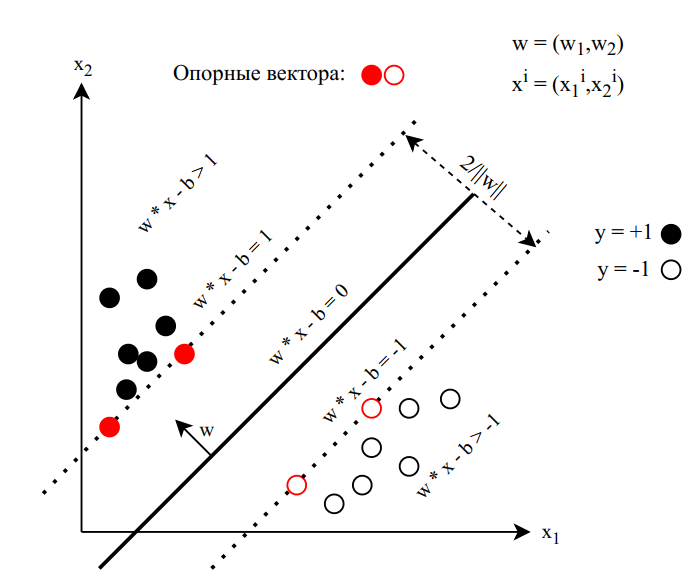
\includegraphics[,scale=0.8]{./img/svm1.png}
		\caption{Принцип работы метода опорных векторов}  
		\label{svm1}
\end{figure}
\newpage
Отклонение $\epsilon$ одно и тоже в силу того, что расстояние до опорных векторов будет одинаковым, иначе такая гиперплоскость точно не будет оптимальной.

После нормировки, а именно поделим вектор c и число d на $\epsilon$, получается:
\begin{equation}
\begin{cases}
(w', x) - b' = 1,\\
(w', x) - b' = -1.
\end{cases}
\end{equation}

Расстояние между двумя параллельными гиперплоскостями можно вычислить следующим образом:
\begin{equation}
    dist = \frac{|b_1 - b_2|}{||w||},
\end{equation}
где $b_1$ --- свободный член первой гиперплоскости, $b_2$ --- свободный член второй гиперплоскости, $||w|| = w \cdot w$ --- одинаков, вследствие параллельности гиперплоскостей.

Тогда несложно убедиться, что расстояние от параллельных гиперплоскостей до оптимальной гиперплоскости равно $\frac{1}{||w||}$. Теперь, чтобы найти оптимальную гиперплоскость, нужно решить следующую задачу оптимизации:
\begin{equation}
    \begin{cases}
    ||w|| \longrightarrow min, \\
    (w, x_i) - b \ge 1, \text{если }  y_i = 1, \\
    (w, x_j) - b \le -1, \text{если }  y_j = -1.
    \end{cases}
\end{equation}

Или в более удобной записи:
\begin{equation}
    \begin{cases}
    ||w|| \longrightarrow min, \\
    y_i \cdot [(w, x_i) - b] \ge 1, y_i \in \{-1; 1\}.
    \end{cases}
\end{equation}

Эта задача сводится к двойственной задаче поиска седловой точки функции Лагранжа. Но если в случае отсутствия линейной разделимости требуется ввести набор дополнительных переменных $\delta_i$, характеризующих величину ошибки на объектах $x_i \in \{x_1, ..., x_n\}$. Тогда задача оптимизации изменится следующим образом:

\begin{equation}
    \begin{cases}
    ||w|| + \sum\delta_i\longrightarrow min, \\
    y_i \cdot [(w, x_i) - b] \ge 1 - \delta_i, y_i \in \{-1; 1\}, \\
    \delta_i \ge 0, i \in \{1, ..., n\}.
    \end{cases}
\end{equation}

Здесь, $\delta_i$ равно нулю в том случае, если соответствующее неравенство выполняется и без него. То есть $\delta_i$ является минимально возможным значением, при котором неравенство будет выполнено. Решая эти задачи, можно получить вектор c, который и нужен для построения гиперплоскости.

Ниже, на рисунке \ref{svm2}, представлен вывод правил настройки весов.
\captionsetup{justification=centering,singlelinecheck=off}
\begin{figure}[h!]
	\centering
		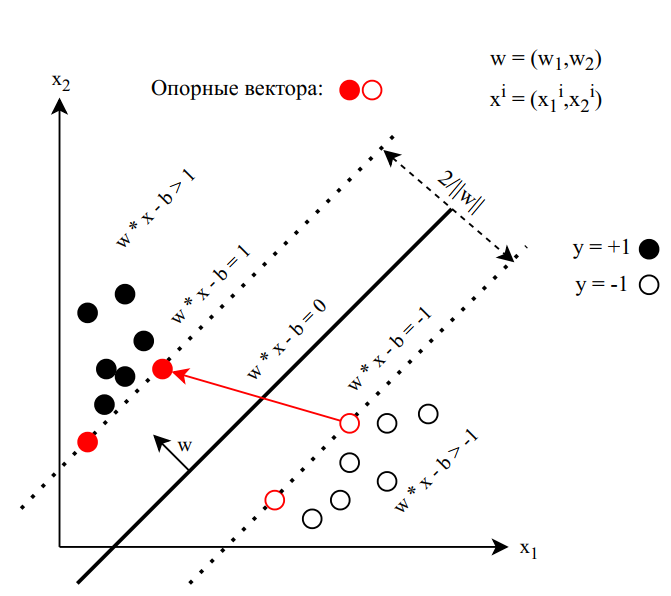
\includegraphics[,scale=0.8]{./img/svm2.png}
		\caption{Вывод правил настройки весов}  
		\label{svm2}
\end{figure}
\newpage
\subsection{Классификации текстов}

На данном этапе обученная модель получает на вход новостной текст. Этот текст необходимо очистить, предварительно обработать и извлечь признаки, используя те же этапы, что и для набора обучающих данных, чтобы получить соответствующие признаки. Входной текст преобразуется в вектор признаков и с помощью обученной модели прогнозирует тематику исходного новостного текста.

\section{Метрики оценки качества классификации текстов}

Показатели критериев оценки качества классификации, будут базироваться на следующих основных метриках результатов классификации на тестовой выборке.

\begin{itemize}[label = ---]
    \item TP (англ. True Positive) –-- истинный положительный результат. Верные данные, классифицированные как верные.
    \item TN (англ. True Negative) –-- истинный отрицательный результат. Неверные данные, классифицированные как неверные.
    \item FP (англ. False Positive) –-- ложный положительный результат. Верные данные, классифицированные как неверные.
    \item FN (англ. False Negative) –-- ложный отрицательный результат. Неверные данные, классифицированные как верные.
\end{itemize}

Для оценки качества модели, обученного на обучающей и тестовой выборках из набора данных, используются следующие две метрики: аккуратность и F1-мера.

Метрики аккуратности (англ. Accuracy) --- один из наиболее простых, а поэтому и распространенной метрикой. Она показывает количество правильно проставленных меток класса (суммы истинно положительных и истинно отрицательных результатов) от общего количества данных и считается следующим образом:
\begin{equation}
    Accuracy = \frac{TP + TN}{TP + TN + FP + FN}.
\end{equation}

F1-мера —-- это показатель оценки, который измеряет качество работы модели классификации. Он сочетает в себе оценки точности и полноты модели.

Точность модели (англ. Precision) —-- это показатель оценки модели и производительности, который соответствует доле значений, которые фактически принадлежат положительному классу, среди всех значений, которые, по прогнозам, принадлежат этому классу. Точность также известна как положительная прогностическая ценность (англ. positive predictive value, PPV). Оценка F1 использует точность, чтобы получить долю истинно положительных записей среди общего числа записей, классифицированных как положительные с помощью модели машинного обучения. Точность модели рассчитывается следующим образом:
\begin{equation}
    Precision = \frac{TP}{TP + FP}.
\end{equation}

Полноты модели (англ. Recall)--- это показатель оценки модели и производительности, который соответствует доле значений, которые, по прогнозам, относятся к положительному классу, среди всех значений, которые действительно принадлежат к положительному классу (включая ложно отрицательные). F1-мера использует полноты, чтобы получить долю истинно положительных записей среди общего числа фактически положительных записей. Полноты модели рассчитывается следующим образом:
\begin{equation}
    Recall = \frac{TP}{TP + FN}.
\end{equation}

Значение F1-меры рассчитывается как гармоническое среднее значений точности и полноты модели, по следующей формуле:
\begin{equation}
    F1 = 2 \cdot \frac{Precision \cdot Recall}{Precision + Recall} = \frac{TP}{TP + \frac{1}{2} (FP + FN)}.
\end{equation}

\section{Функциональная схема обучения модели}

Для обучения модели используется метод SVM, а для метода извлечения признаков из набора текстов используется метод TF-IDF. На входе поступает набор новостных текстов с соответствующей меткой для обучения, а на выходе --- обученная модель на этом наборе.

Ниже, на рисунке \ref{2-train} представлена функциональная схема обучения модели (с помощью SVM) в виде IDEF0-диаграммы. На этой схеме отображены этапы создания обучающей и тестовой выборок, очистки и предобработки текстов, извлечения признаков и выполнения многоклассовой классификации для обучающей
выборки.

\captionsetup{justification=centering,singlelinecheck=off}
\begin{figure}[h!]
	\centering
		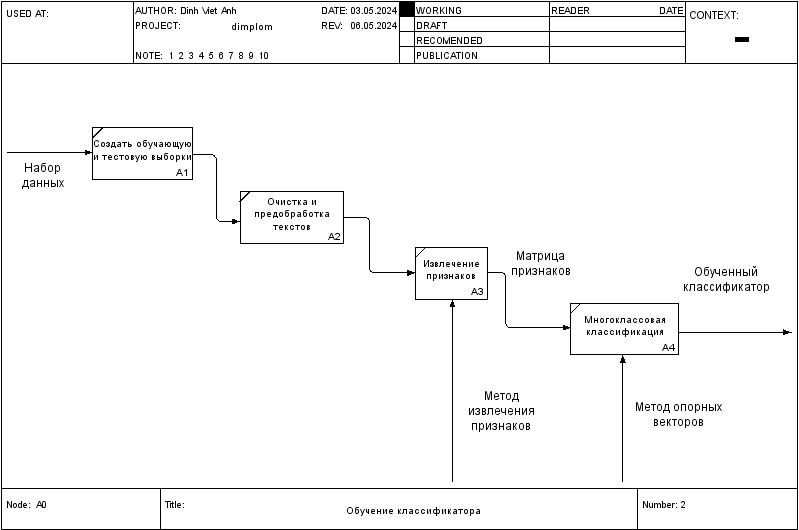
\includegraphics[,scale=0.55]{./img/train.png}
		\caption{Функциональная схема обучения модели}  
		\label{2-train}
\end{figure}
\newpage
\section{Функциональная схема метода классификации}

Ниже, на рисунке \ref{2-use} представлена функциональная схема метода классификации в виде IDEF0-диаграммы. На входе поступает новостной текст для классификации, а выходе --- прогнозируемое название тематика этого текста. 

На этой схеме отображены этапы очистки и предобработки входного текста, извлечения признаков и выполнения распознавания тематика текста, использующего обученную модель.

\captionsetup{justification=centering,singlelinecheck=off}
\begin{figure}[h!]
	\centering
		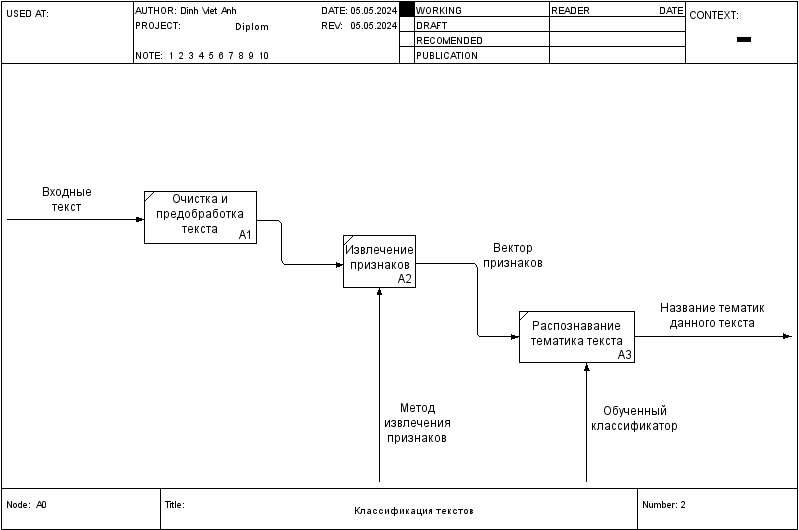
\includegraphics[,scale=0.55]{./img/use.png}
		\caption{Функциональная схема метода классификации}  
		\label{2-use}
\end{figure}
\newpage
\section{Описание используемого набора данных}

Для обучения модели было решено использовать набор данных News dataset from Lenta.Ru \cite{kaggle_data}. Этот набор данных содержит более 800 тысяч новостей на русском языке, соответствующих более чем 20 тематикам, с сентября 1999 года по декабрь 2019 года. Источник новостей —-- сайт lenta.ru \cite{lenta}, российское новостное интернет-издание, основанное в 1999 году. В наборе данных для каждой новости сохраняются текст, заголовок, тематик, дата публикации и ссылка на источник. Этот набор данных можно скачать с сайта Кaggle \cite{kaggle} --- система организации конкурсов по исследованию данных, а также социальная сеть специалистов по обработке данных и машинному обучению. 

После скачивания набора данных необходимо выполнить этап фильтрации данных, чтобы сохранить набор данных в виде файла CSV и создать наборы обучения для будущего использования.

Ниже, на рисунке \ref{2-file}, представлены примеры некоторых строк в наборе данных.

\captionsetup{justification=centering,singlelinecheck=off}
\begin{figure}[h!]
	\centering
		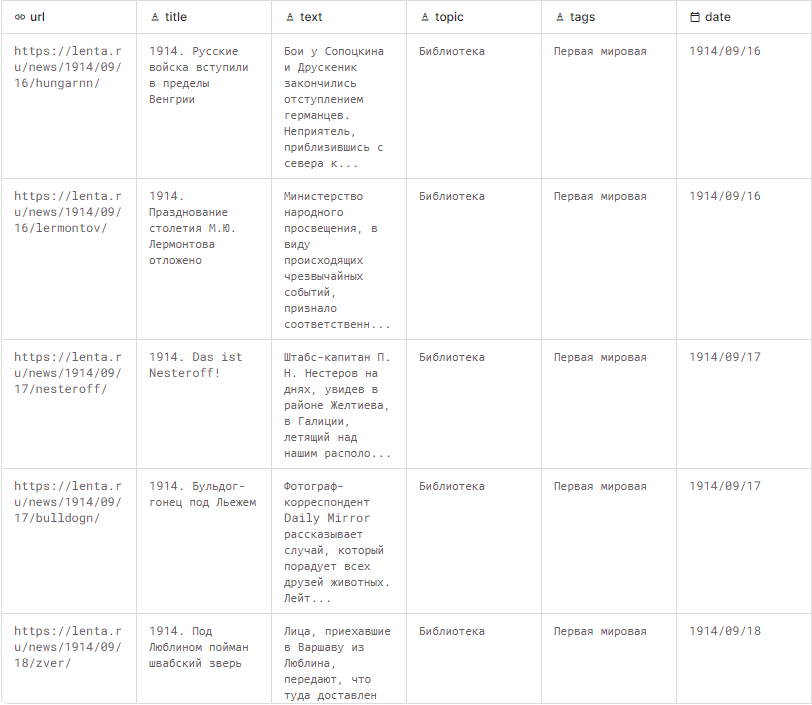
\includegraphics[,scale=0.75]{./img/file.png}
		\caption{Примеры некоторых строк в наборе данных}  
		\label{2-file}
\end{figure}
\newpage


\section*{Вывод}

В этом разделе были описаны этапы работы алгоритма разрабатываемого метода, также были рассмотрены функциональные схемы обучения модели и метод классификации. Также были приведены метрики, используемые для оценки качества работы обученного модели. Был описан используемый набор данных для обучения модели и была рассмотрена структура программного обеспечения.